%*******************************************************************************
%*********************************** First Introduction *****************************
%*******************************************************************************
%\chapter{Introduction}  %Title of the First Introduction
%\chapter*{Introduction}
\chapter{Introduction}  %Title of the First Introduction
%\addcontentsline{tableofcontents}{chapter}{introduction}

\ifpdf
    \graphicspath{{Introduction/Figs/Raster/}{Introduction/Figs/PDF/}{Introduction/Figs/}}
\else
    \graphicspath{{Introduction/Figs/Vector/}{Introduction/Figs/}}
\fi


%********************************** %First Section  **************************************
\section{Motivation}\label{section1.1} %Section - 1.1 
\emph{Text mining} is the process of searching for patterns in natural language text using methods in computer science, linguistics, and statistics. Despite being unstructured and only human-understandable, text is still our primary media for exchange of information\cite{witten2005text}. The prevalence of textual data presents a big challenge to computer-driven natural language understanding. \emph{Information extraction}, in particular, refers to the task of acquiring organized, structured and queryable format of data from the unstructured corpus. \newline\newline
While text mining is widely used in areas like marketing and document verifying, it has received increased attention for its application to biomedical literatures\cite{kim2003genia,ananiadou2006text,krallinger2005text}. This trend stems from the direct need of biomedical workers and researchers to cope with information explosion in their field. For instance, MEDLINE(Medical Literature Analysis and Retrieval System Online), the online database of United States National Library of Medicine, has accumulated nearly 0.8 million citations and 2.7 billion searches in 2014 alone\cite{MEDLINE:2015:Online}, with total citations reaching 25 million. Within these publications there are valuable research results that should add to human knowledge. In the meantime,  our primary knowledge base in life science - the biomedical databases, are still mostly being populated manually by \emph{biocurators} - the ``museum catalogers of the Internet age''\cite{wiki:biocurators}. They are professional scientists who read biomedical articles, record relevant data and organize them according to the biomedical database schema. The sheer volume of publications has made this process increasingly unrealistic\cite{cohen2005survey}.\newline\newline
Not only does data overload make knowledge discovery demanding, it also leads to a decline in literature quality. Nowadays biomedical workers and researchers are more prone to drawing wrong conclusions because they simply can not read all the relevant publications, among which oftentimes contradicting results are reported. Needless to say, we are in desperate need of automatic tools for systematically analyzing documents and extracting information. In fact, it has been argued that text mining is required to improve the coverage of databases\cite{baumgartner2007manual}.

%********************************** %Second Section  *************************************
\section{Definitions and Assumptions}\label{section1.2}%Section - 1.2
Below are a list of terms which I will use throughout this thesis, more detailed examples will be given in the relevant sections, but a general definition is first given here to avoid any confusions that might arise.
\begin{itemize}
		\begin{figure}[h]
			\centering
			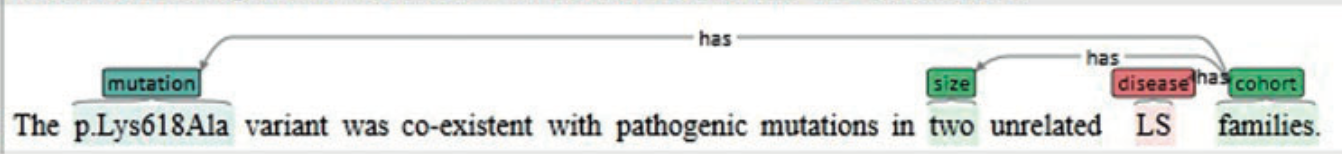
\includegraphics[width=\textwidth]{Relations_Example}
			\caption{An Example of Relations Captured in a Sentence}
			\label{fig:Relations_Example}   
		\end{figure}
	\item \emph{Relation Extraction:} In general, relation extraction refers to the process of discovering a relationship between entities in text. Relations can be unary (one-to-itself), binary (one-to-one) and more complex\cite{mcdonald2005simple}. In this project we are mainly concerned with binary relations between two entities. As illustrated in Figure \ref{fig:Relations_Example}, the sentence contains relations like \emph{families have p.Lys618A1a}, \emph{families have two(members)}, \emph{families have the LS(disease)}, etc. In the domain of natural language processing, the relation can be semantic or syntactic, with semantic relations being the most important for knowledge discovery. Specifically, semantic relations between biomedical entities such as protein-protein interactions and gene expressions cover a wide range of knowledge in this field and have driven numerous research work.
	\begin{figure}[h]
		\centering
		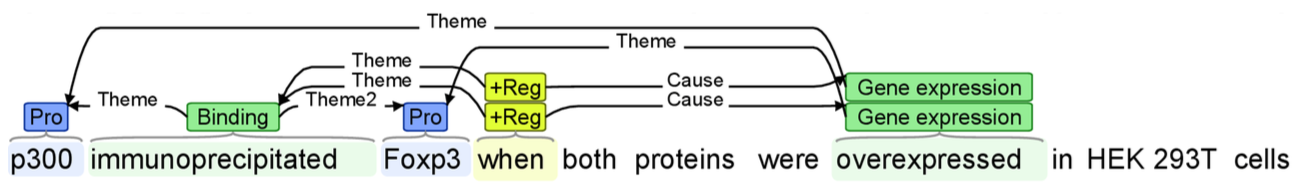
\includegraphics[width=\textwidth]{Events_Example}
		\caption{An Example of Events Captured in a Sentence}
		\label{fig:Events_Example}   
	\end{figure}
	\item \emph{Event Extraction:} A biomedical event usually refers to a statement of molecular interaction in text \cite{bjorne2011generalizing}. Figure \ref{fig:Events_Example} shows a sentence that contains two protein catabolism events (pro), one binding event, two positive regulation events, and two gene expression events between respective entities.
\end{itemize}
Both relation extraction and event extraction belongs to the broader concept of information extraction.

%********************************** % Third Section  *************************************
\section{Research Question}\label{section1.3} %Section - 1.3
This project looks to investigate the adaptation of event extraction system Approximate Subgraph Matching (ASM)\cite{liu2013approximate},  on relation extraction tasks, specifically regarding the relations in the Variome Corpus annotated with the Variome Annotation Schema\cite{verspoor2013annotating}. The effectiveness of the system in extracting relations between entities (disease, ethnicity, gender, gene, mutation, patient, etc.) will be evaluated. Since ASM is a supervised, rule-based data mining system developed solely for event extraction, it needs to be re-trained and carefully adapted to the new corpus. We believe such a relation extraction tool has very promising applications for biomedical researchers, doctors, pharmaceutical companies, and the general public. The extracted relations can be helpful in information search, knowledge discovery and hypothesis generation. 
%In this project we focus on the relation extraction among other informations. Biomedical relations covers a wide range of knowledge in this field. As it turns out, this is not a trivial process, 
\section{Thesis Structure}
The remainder of the thesis is organized in the following manner. In Chapter 2, we discuss different algorithms used for relation extraction tasks including pattern-based methods, co-occurrence based methods, feature-based methods, semi-supervised methods and kernel based methods. In Chapter 3, we provide a detailed description of the Approximate Subgraph Matching system and explain how this event extraction system was adapted for relation extraction task in Variome Corpus. We then present the relation extraction results and our analysis. In Chapter 4, we conclude our work and present future directions.

